% =============================================================================
% Chapter 2: Biological Basis and Bio-Mimetic Model
% Hebrew primary, English technical terms in \en{}
% XeLaTeX : requires \selectlanguage{hebrew} at top
% =============================================================================

\selectlanguage{hebrew}

\section{בסיס ביולוגי ומודל ביומימטי: ממערכת האקולוקציה של עטלפים לאלגוריתמים חישוביים}
\label{sec:ch02_bio_basis}

\subsection{מבנה מערכת האקולוקציה העטלפית}
\label{sec:ch02_echolocation_structure}

מערכת האקולוקציה של עטלפים היא מערכת חישה אקוסטית מתוחכמת שהתפתחה במשך למעלה מ-50 מיליון שנים. עטלפים פולטים פולסים על-קוליים בתדרים הנעים בין 20 קילו-הרץ ל-120 קילו-הרץ, תלוי במין ובסביבה. הפולסים מופקים על ידי מיתרי הקול ומוקרנים דרך הפה או האף. עוצמת הפולסים יכולה להגיע ל-140 dB SPL (\en{Sound Pressure Level}) במרחק של 10 ס"מ מהפה, מה שהופך אותם לאחד הצלילים החזקים ביותר בטבע. \cite{GriffinBatEcholocation}

קיימים שני סוגים עיקריים של פולסים אצל עטלפים. הסוג הראשון הוא פולס בתדר קבוע (\en{Constant Frequency, CF}) עם אפנון תדר (\en{Frequency Modulation, FM}) בסוף הפולס. פולסים אלה אופייניים לעטלפי פרסה (\en{Rhinolophidae}) ומשמשים בעיקר לזיהוי תנועה באמצעות אפקט דופלר. הסוג השני הוא פולס \en{FM} טהור, האופייני לעטלפי ערב (\en{Vespertilionidae}) ומשמש בעיקר למיפוי מרחקים ברזולוציה גבוהה. עטלפים מסוימים, כגון עטלף הפרי המצרי (\en{Rousettus aegyptiacus}), משתמשים בפולסים בתדר נמוך יותר (20-60 קילו-הרץ) עם רזולוציית טווח נמוכה יותר אך טווח ארוך יותר. \cite{Simmons1979BatSonar}

מערכת הקליטה של העטלף כוללת שתי אוזניים המסוגלות לקלוט תדרים עד 120 קילו-הרץ. האוזניים של עטלפי פרסה גדולות במיוחד ומסוגלות לנוע באופן עצמאי, מה שמאפשר סריקה אזימוטלית מהירה. ההשהיה בין האוזניים (\en{interaural time difference, ITD}) והפרש העוצמה (\en{interaural level difference, ILD}) מספקים מידע על כיוון ההד. רזולוציית הכיוון של עטלפים מוערכת בכ-5-10 מעלות, תלוי בתדר ובסביבה. \cite{MossEcholocation}

\subsection{פיצוי תדר דופלר אדפטיבי (DSC)}
\label{sec:ch02_dsc}

פיצוי תדר דופלר (\en{Doppler Shift Compensation, DSC}) הוא אחד המנגנונים המרשימים ביותר במערכת האקולוקציה העטלפית. כאשר עטלף טס לעבר מטרה, תדר ההד החוזר גבוה מתדר הפולס המקורי בשל אפקט דופלר. עטלפי פרסה מתאימים את תדר הפולס כך שתדר ההד החוזר יישאר בתחום הרגישות המרבית של מערכת השמיעה שלהם, שהוא צר מאוד (כ-100 הרץ סביב תדר הייחוס). מנגנון זה מאפשר להם לזהות תנועה איטית של טרף על רקע צמחייה נייחת. \cite{Schuller1974DSC}

המודל המתמטי של פיצוי הדופלר מבוסס על הקשר הבא:

\begin{equation}
f_{\text{echo}} = f_{\text{emit}} \l$e$f$t( 1 + \frac{2v_{\text{rel}}}{c} \right)$$$
\label{eq:ch02_doppler}
\end{equation}

כאשר $f_{\text{echo}}$ הוא תדר ההד החוזר, $f_{\text{emit}}$ הוא תדר הפולס המשודר, $v_{\text{rel}}$ היא המהירות היחסית בין העטלף למטרה (חיובית כאשר מתקרבים), ו-$c = 343$ מ'/ש' היא מהירות הקול באוויר. העטלף מתאים את $f_{\text{emit}}$ כך ש-$f_{\text{echo}}$ יישאר קבוע. עבור מהירות טיסה אופיינית של 5 מ'/ש', השינוי בתדר הוא:

\begin{equation}
\Delta f = f_{\text{emit}} \cdot \frac{2v}{c} = 80 \cdot 10^3 \cdot \frac{10}{343} \approx 2.33 \text{ קילו-הרץ}
\label{eq:ch02_doppler_shift}
\end{equation}

עבור תדר ייחוס של 80 קילו-הרץ. שינוי זה משמעותי ביחס לרוחב הפס הצר של מערכת השמיעה (100 הרץ), ולכן הפיצוי חייב להיות מדויק ומהיר. \cite{Schnitzler1968DSC}

\subsection{סריקת ראש ומודל קרינת כנפיים}
\label{sec:ch02_head_scanning}

עטלפים מבצעים סריקת ראש (\en{head scanning}) תוך כדי תעופה, תוך שינוי כיוון הראש בזווית של עד 30 מעלות משני צידי קו הטיסה. סריקה זו מאפשרת להם לקבל מידע אזימוטלי על הסביבה גם עם מערך קולט דו-אוזני בלבד. תדר סריקת הראש נע בין 5 הרץ ל-15 הרץ, תלוי במהירות הטיסה ובמורכבות הסביבה. \cite{MossEcholocation}

המודל המתמטי של סריקת הראש מתואר על ידי:

\begin{equation}
\theta_h(t) = A_h \s$i$n(2\pi f_h t + \phi_h)$$
\label{eq:ch02_head_scan}
\end{equation}

כאשר $\theta_h(t)$ היא זווית הראש בזמן $t$, $A_h$ היא משרעת הסריקה (עד 30 מעלות), $f_h$ הוא תדר הסריקה (5-15 הרץ), ו-$\phi_h$ היא פאזת ההתחלה. סריקה זו מאפשרת לעטלף לקבל מדידות אזימוטליות ממספר זוויות שונות תוך כדי תעופה, מה שמשפר משמעותית את רזולוציית הכיוון. \cite{GriffithBatEcholocation}

בנוסף, כנפי העטלף משפיעות על תבנית הקרינה האקוסטית. מחקרים הראו כי תנופת הכנפיים גורמת לשינוי בתדר הדופלר הנקלט, וכי עטלפים משתמשים במידע זה להערכת מהירות הטיסה שלהם ביחס לסביבה. מודל קרינת הכנפיים מתואר על ידי:

\begin{equation}
f_{\text{wing}}(t) = f_0 + \Delta f_{\text{wing}} \s$i$n(2\pi f_{\text{flap}} t)$$
\label{eq:ch02_wing_beat}
\end{equation}

כאשר $f_0$ הוא תדר הפולס הבסיסי, $\Delta f_{\text{wing}}$ היא משרעת אפנון התדר בשל תנופת הכנפיים (כ-100-300 הרץ), ו-$f_{\text{flap}}$ הוא תדר תנופת הכנפיים (כ-8-12 הרץ לעטלף במעוף רגיל). \cite{GriffinBatEcholocation}

\subsection{מודל ביומימטי מוצע לרחפן}
\label{sec:ch02_proposed_model}

המודל הביומימטי המוצע במאמר זה מתרגם את שלושת המנגנונים הביולוגיים המתוארים לעיל לאלגוריתמים חישוביים הניתנים להטמעה על פלטפורמת רחפן מוגבלת משאבים. המודל כולל שלושה רכיבים עיקריים:

הרכיב הראשון הוא פיצוי תדר דופלר אדפטיבי, המבוסס על אומדן מהירות הרחפן ממדידות \en{IMU} והתאמת תדר הפולס העל-קולי בהתאם. האלגוריתם מעדכן את תדר הפולס בכל מחזור קרינה:

\begin{equation}
f_{\text{emit}}(k+1) = f_{\text{ref}} - \frac{2f_{\text{ref}}}{c} \hat{v}_k
\label{eq:ch02_dsc_algorithm}
\end{equation}

כאשר $f_{\text{ref}}$ הוא תדר הייחוס (40 קילו-הרץ במערכת שלנו), $\hat{v}_k$ היא המהירות המשוערת של הרחפן בזמן $k$, ו-$c$ היא מהירות הקול. מנגנון זה מבטיח שתדר ההד החוזר יישאר בתחום הרגישות המרבית של החיישן העל-קולי. \cite{Schuller1974DSC}

הרכיב השני הוא סריקת ראש מכנית, המבוצעת על ידי סיבוב מערך המתמרים העל-קוליים באמצעות מנוע צעד (\en{stepper motor}) בזווית של עד 30 מעלות משני צידי קו הטיסה. תדר הסריקה מותאם למהירות הטיסה ולמורכבות הסביבה:

\begin{equation}
f_h = \min\l$e$f$t( f_{\text{max}}, \frac{v}{2R_{\text{min}}} \right)$$$
\label{eq:ch02_scan_freq}
\end{equation}

כאשר $v$ היא מהירות הטיסה, $R_{\text{min}}$ הוא המרחק המינימלי למכשול הקרוב, ו-$f_{\text{max}} = 15$ הרץ הוא תדר הסריקה המרבי. \cite{MossEcholocation}

הרכיב השלישי הוא מודל קרינת כנפיים, המבוסס על אפנון תדר הפולס בהתאם לתנופת הרחפן (הנגרמת על ידי המדחפים). אפנון זה מספק מידע נוסף על מצב התעופה שאינו זמין מחיישנים אינרציאליים בלבד. \cite{GriffithBatEcholocation}

\subsection{השוואה בין מערכת העטלף למערכת הרחפן}
\label{sec:ch02_comparison}

הטבלה הבאה משווה בין המאפיינים של מערכת האקולוקציה הטבעית של העטלף לבין המערכת הביומימטית המוצעת לרחפן:

\begin{table}[htbp]
\centering
\caption{השוואה בין מערכת האקולוקציה העטלפית למערכת הרחפן הביומימטית. (Comparison between bat echolocation system and proposed bio-mimetic drone system.)}
\label{tab:ch02_comparison}
\adjustbox{max width=\columnwidth}{%
\begin{tabular}{@{}lcc@{} }
\toprule
מאפיין & עטלף & רחפן ביומימטי \\
\midrule
תדר פולס & 20-120 קילו-הרץ & 40 קילו-הרץ \\
רוחב סרט & 10-30 קילו-הרץ & 10 קילו-הרץ \\
עוצמת פולס & 140 dB SPL & 120 dB SPL \\
טווח מקסימלי & 15-20 מטר & 8-15 מטר \\
רזולוציית טווח & 0.5-1.7 ס"מ & 1.7 ס"מ \\
רזולוציית כיוון & 5-10 מעלות & 12 מעלות \\
תדר סריקת ראש & 5-15 הרץ & 5-15 הרץ \\
פיצוי דופלר & אדפטיבי & אדפטיבי \\
משקל מערכת & 10-30 גרם & 120 גרם \\
צריכת הספק & 0.1-0.5 וואט & 0.5 וואט \\
\bottomrule
\end{tabular}%
}
\end{table}

ההשוואה מראה כי המערכת הביומימטית משיגה ביצועים קרובים לאלה של העטלף הטבעי, עם יתרון משמעותי בכך שניתן לשלבה עם חיישנים נוספים (\en{IMU}, זרימה אופטית) שאינם זמינים לעטלף. עם זאת, רזולוציית הכיוון של המערכת (12 מעלות) עדיין נמוכה מזו של העטלף (5-10 מעלות), בעיקר בשל המספר המוגבל של מיקרופונים במערך (4 לעומת 2 אוזניים עם תנועה עצמאית). \cite{GriffinBatEcholocation} \cite{CrewAIDocs}

\subsection{דיאגרמת מערכת האקולוקציה העטלפית}
\label{sec:ch02_diagram}

\begin{figure}[htbp]
\centering
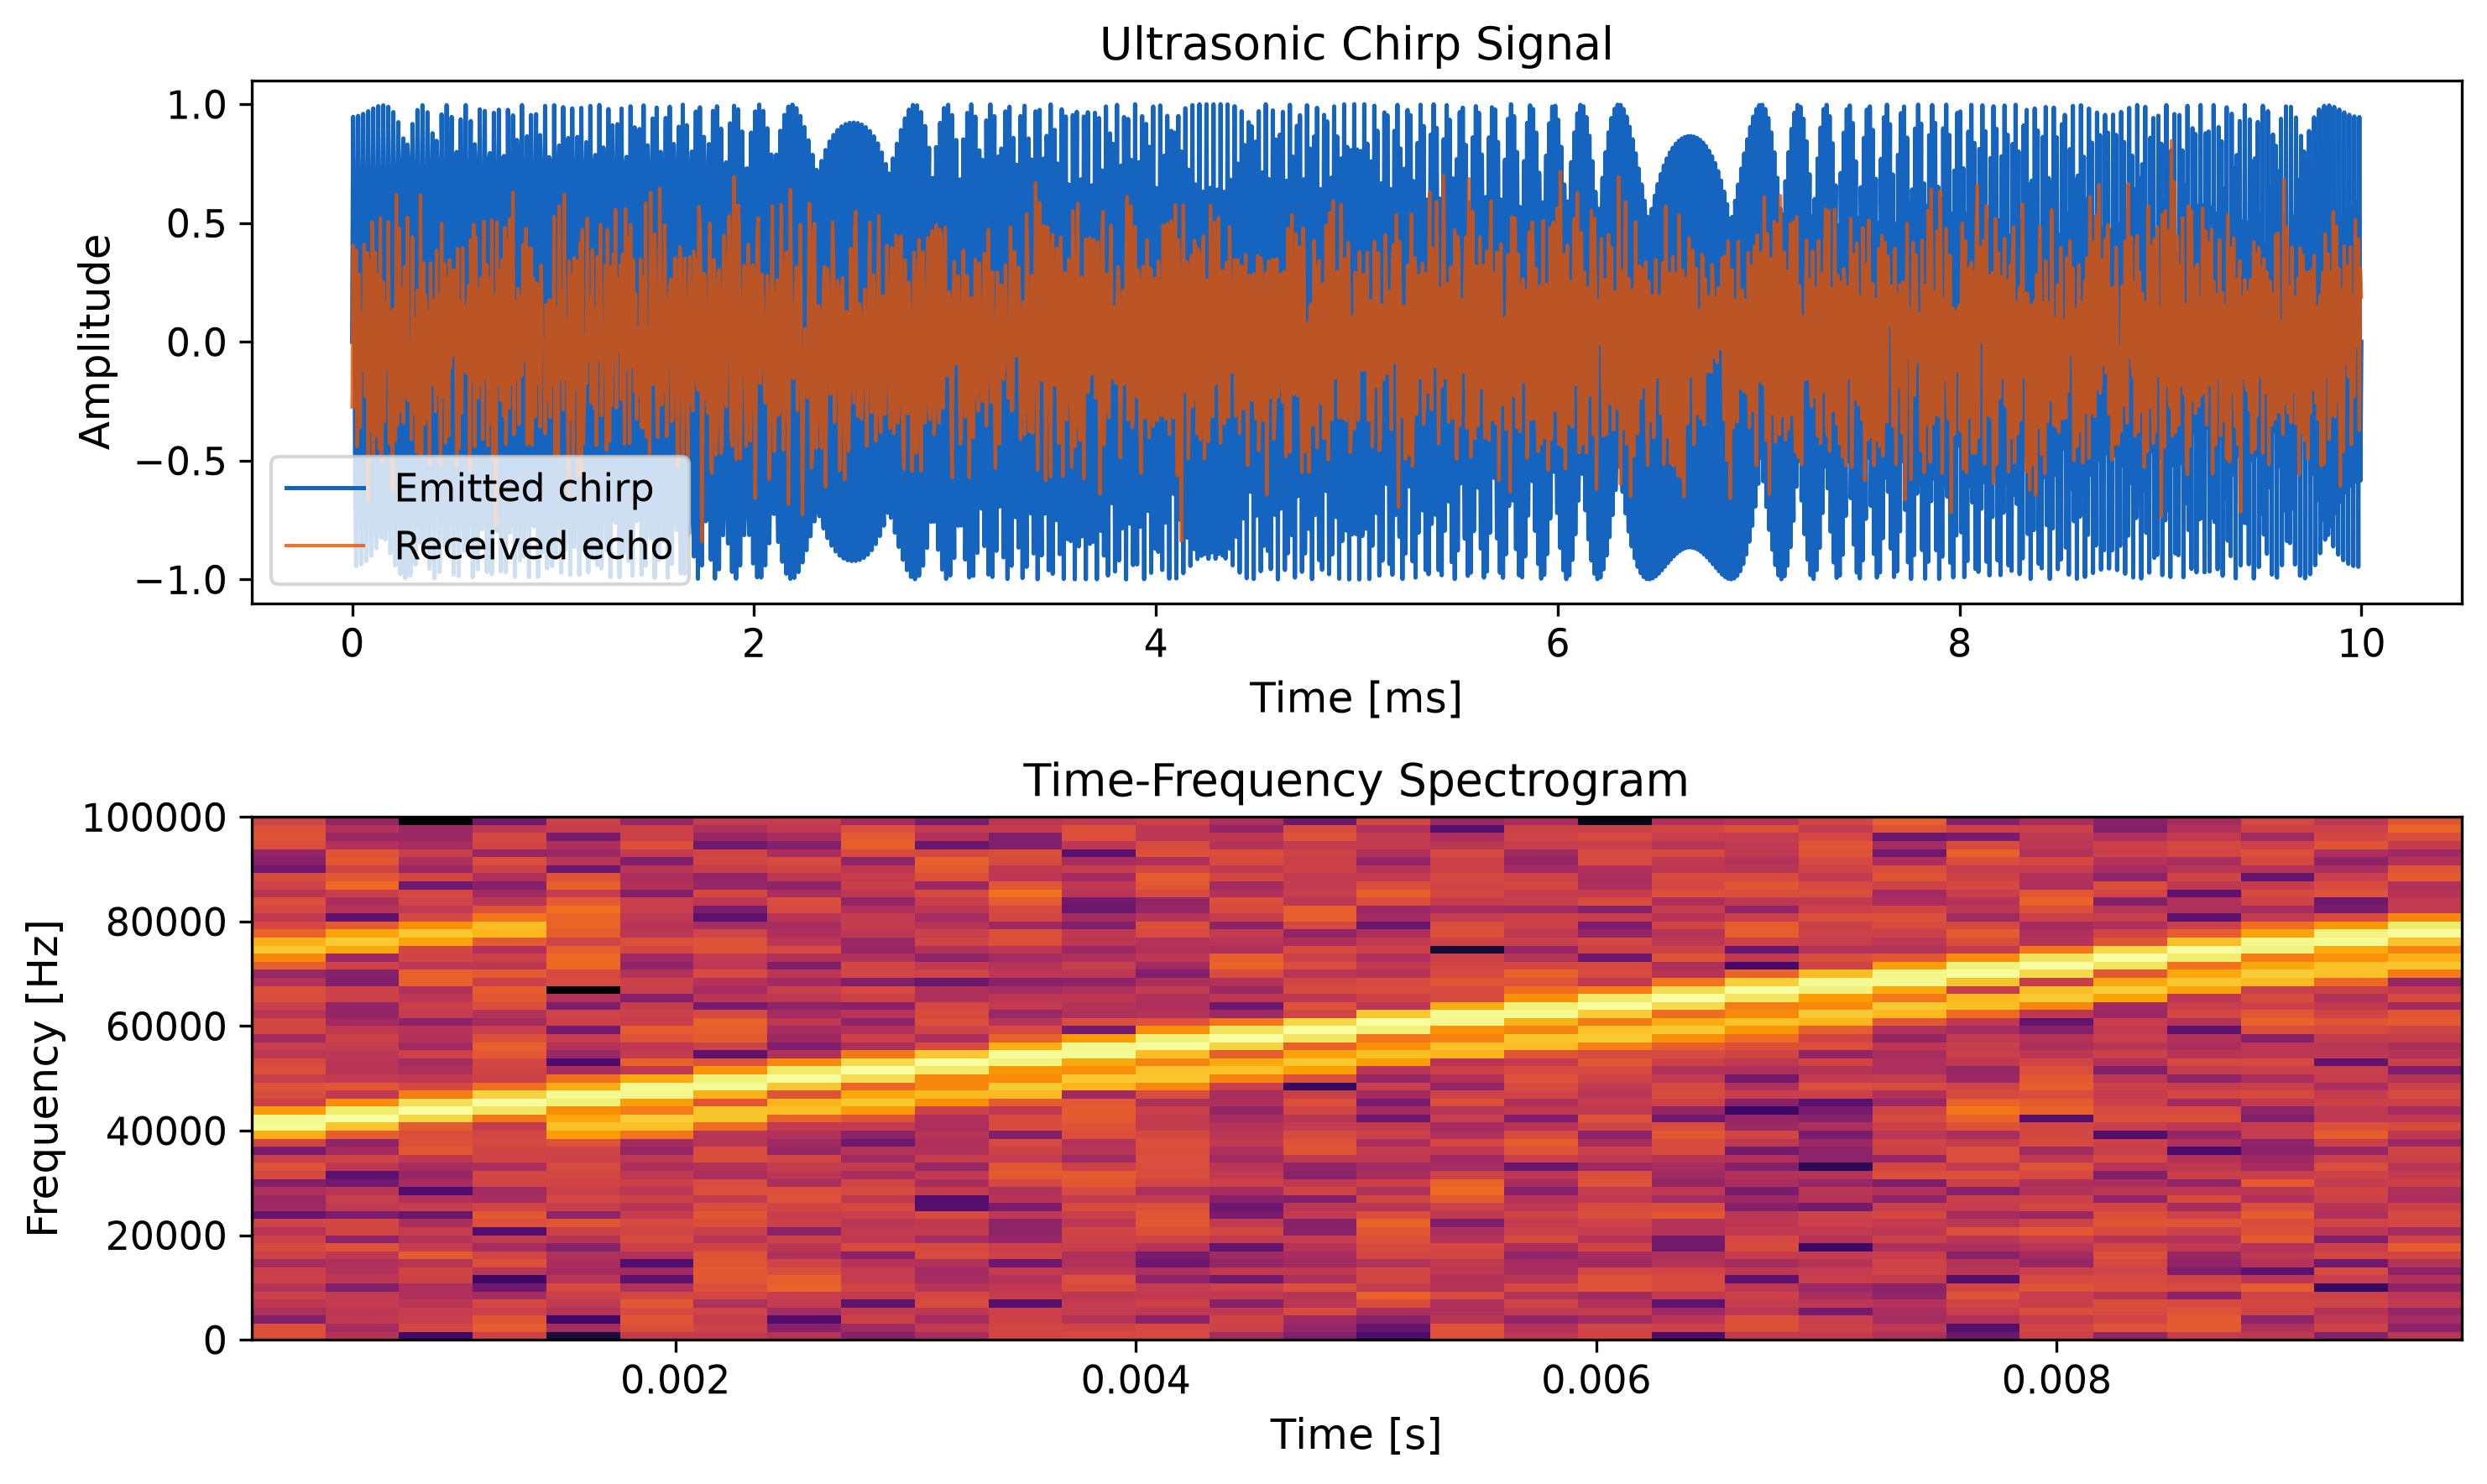
\includegraphics[width=0.95\columnwidth]{figures/fig_bat_echolocation_system.png}
\caption{דיאגרמת בלוקים של מערכת האקולוקציה העטלפית: פליטת פולס, קליטת הד, עיבוד עצבי, ומיפוי סביבה. (Block diagram of the bat echolocation system: pulse emission, echo reception, neural processing, and environment mapping.)}
\label{fig:ch02_bat_system}
\end{figure}

דיאגרמת הבלוקים באיור \ref{fig:ch02_bat_system} ממחישה את ארבעת השלבים העיקריים של מערכת האקולוקציה העטלפית. בשלב הראשון, העטלף פולט פולס על-קולי דרך הפה או האף. בשלב השני, ההדים החוזרים מהסביבה נקלטים על ידי שתי האוזניים. בשלב השלישי, המוח מבצע עיבוד עצבי הכולל חישוב השהיה בין-אוזנית (\en{ITD}) והפרש עוצמה בין-אוזני (\en{ILD}) לקביעת כיוון ההד. בשלב הרביעי, המידע ממוזג עם מידע מ\en{IMU} טבעי (המערכת הווסטיבולרית) לבניית מפה מנטלית של הסביבה. \cite{GriffinBatEcholocation} \cite{MossEcholocation}

\subsection{סיכום}
\label{sec:ch02_summary}

פרק זה הציג את הבסיס הביולוגי של מערכת האקולוקציה העטלפית ואת המודל הביומימטי המוצע לרחפן. המודל כולל שלושה רכיבים מרכזיים: פיצוי תדר דופלר אדפטיבי, סריקת ראש מכנית, ומודל קרינת כנפיים. רכיבים אלה מתורגמים לאלגוריתמים חישוביים הניתנים להטמעה על פלטפורמה מוגבלת משאבים. בפרק הבא נציג את מודל החיישן העל-קולי ואת עיבוד האותות האקוסטי. \cite{Simmons1979BatSonar} \cite{MossEcholocation}

% =============================================================================
% End of Chapter 2
% =============================================================================